%{{第六十八回}}{第六十八回}}

\chapter{苦尤娘赚入大观园\\酸凤姐大闹宁国府}

{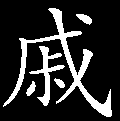
\includegraphics[width=3mm]{../Images/00005}\kaishu 余读《左氏》见郑庄,读《后汉》见魏武,谓古之大奸巨滑,惟此为最。今读《石头记》,又见凤姐作威作福,用柔用刚,占步高,留步宽,杀得死,救得活。天生此等人,斲丧元气不少!}

话说贾琏起身去后,偏值平安节度巡边在外,约一个月方回。贾琏未得确信,只得住在下处等候。及至回来相见,将事办妥,回程已是将两个月的限了。

谁知凤姐心下早已算定,只待贾琏前脚走了,回来便传各色匠役,收拾东厢房三间,照依自己正室一样装饰陈设。至十四日便回明贾母王夫人,说十五日一早要到姑子庙进香去。只带了平儿、丰儿、周瑞媳妇、旺儿媳妇四人,未曾上车,便将原故告诉了众人。又吩咐众男人,素衣素盖,一径前来。

兴儿引路,一直到了二姐门前扣门。鲍二家的开了。兴儿笑说:``快回二奶奶去,大奶奶来了。''鲍二家的听了这句,顶梁骨走了真魂,忙飞进报与尤二姐。尤二姐虽也一惊,但已来了,只得以礼相见,于是忙整衣迎了出来。至门前,凤姐方下车进来。尤二姐一看,只见头上皆是素白银器,身上月白缎袄,青缎披风,白绫素裙。眉弯柳叶,高吊两梢,目横丹凤,神凝三角。俏丽若三春之桃,清洁若九秋之菊。周瑞旺儿二女人搀入院来。尤二姐陪笑忙迎上来万福,张口便叫:``姐姐下降,不曾远接,望恕仓促之罪。''说着便福了下来。凤姐忙陪笑还礼不迭。二人携手同入室中。

凤姐上座,尤二姐命丫鬟拿褥子来便行礼,说:``奴家年轻,一从到了这里之事,皆系家母和家姐商议主张。今日有幸相会,若姐姐不弃奴家寒微,凡事求姐姐的指示教训。奴亦倾心吐胆,只伏侍姐姐。''说着,便行下礼去。凤姐儿忙下座以礼相还,口内忙说:``皆因奴家妇人之见,一味劝夫慎重,不可在外眠花卧柳,恐惹父母担忧。此皆是你我之痴心,怎奈二爷错会奴意。眠花宿柳之事瞒奴或可,今娶姐姐二房之大事亦人家大礼,亦不曾对奴说。奴亦曾劝二爷早行此礼,以备生育。不想二爷反以奴为那等嫉妒之妇,私自行此大事,并不说知。\elegantpar{使奴有冤难诉,惟天地可表。}{能装蒜}前于十日之先奴已风闻,恐二爷不乐,遂不敢先说。今可巧远行在外,故奴家亲自拜见过,还求姐姐下体奴心,起动大驾,挪至家中。你我姊妹同居同处,彼此合心谏劝二爷,慎重世务,保养身体,方是大礼。若姐姐在外,奴在内,虽愚贱不堪相伴,奴心又何安。再者,使外人闻知,亦甚不雅观。二爷之名也要紧,倒是谈论奴家,奴亦不怨。所以今生今世奴之名节全在姐姐身上。那起下人小人之言,未免见我素日持家太严,背后加减些言语,自是常情。姐姐乃何等样人物,岂可信真。若我实有不好之处,上头三层公婆,中有无数姊妹妯娌,况贾府世代名家,岂容我到今日。今日二爷私娶姐姐在外,若别人则怒,我则以为幸。正是天地神佛不忍我被小人们诽谤,故生此事。我今来求姐姐进去和我一样同居同处,同分同例,同侍公婆,同谏丈夫。喜则同喜,悲则同悲,情似亲妹,和比骨肉。不但那起小人见了,自悔从前错认了我,就是二爷来家一见,他作丈夫之人,心中也未免暗悔。所以姐姐竟是我的大恩人,使我从前之名一洗无馀了。若姐姐不随奴去,奴亦情愿在此相陪。奴愿作妹子,\elegantpar{每日伏侍姐姐梳头洗面}{谁敢让她梳头洗面}。只求姐姐在二爷跟前替我好言方便方便,容我一席之地安身,奴死也愿意。''说着,便呜呜咽咽哭将起来。尤二姐见了这般,也不免滴下泪来。

二人对见了礼,分序座下。平儿忙也上来要见礼。尤二姐见他打扮不凡,举止品貌不俗,料定是平儿,连忙亲身挽住,只叫:``妹子快休如此,你我是一样的人。''凤姐忙也起身笑说:``折死他了!妹子只管受礼,他原是咱们的丫头。以后快别如此。''说着,又命周家的从包袱里取出四匹上色尺头,四对金珠簪环为拜礼。尤二姐忙拜受了。二人吃茶,对诉已往之事。凤姐口内全是自怨自错,``怨不得别人,如今只求姐姐疼我''等语。尤二姐见了这般,便认他作是个极好的人,小人不遂心诽谤主子亦是常理,故倾心吐胆,叙了一回,竟把凤姐认为知己。又见周瑞等媳妇在旁边称扬凤姐素日许多善政,只是吃亏心太痴了,惹人怨,又说``已经预备了房屋,奶奶进去一看便知。''尤氏心中早已要进去同住方好,今又见如此,岂有不允之理,便说:``原该跟了姐姐去,只是这里怎样?''凤姐儿道:``这有何难,姐姐的箱笼细软只管着小厮搬了进去。这些粗笨货要他无用,还叫人看着。姐姐说谁妥当就叫谁在这里。''尤二姐忙说:``今日既遇见姐姐,这一进去,凡事只凭姐姐料理。我也来的日子浅,也不曾当过家,世事不明白,如何敢作主。这几件箱笼拿进去罢。我也没有什么东西,那也不过是二爷的。''凤姐听了,便命周瑞家的记清,好生看管着抬到东厢房去。于是催着尤二姐穿戴了,二人携手上车,又同坐一处,又悄悄的告诉他:``我们家的规矩大。这事老太太一概不知,倘或知二爷孝中娶你,管把他打死了。如今且别见老太太、太太,我们有一个花园子极大,姊妹住着,容易没人去的。你这一去且在园里住两天,等我设个法子回明白了,那时再见方妥。''尤二姐道:``任凭姐姐裁处。''那些跟车的小厮们皆是预先说明的,如今不去大门,只奔后门而来。

下了车,赶散众人。凤姐便带尤氏进了大观园的后门,来到李纨处相见了。彼时大观园中十停人已有九停人知道了,今忽见凤姐带了进来,引动多人来看问。尤二姐一一见过。众人见他标致和悦,无不称扬。凤姐一一的吩咐了众人:``都不许在外走了风声,若老太太、太太知道,我先叫你们死。''园中婆子丫鬟都素惧凤姐的,又系贾琏国孝家孝中所行之事,知道关系非常,都不管这事。凤姐悄悄的求李纨收养几日,``等回明了,我们自然过去的。''李纨见凤姐那边已收拾房屋,况在服中,不好倡扬,自是正理,只得收下权住。凤姐又变法将他的丫头一概退出,又将自己的一个丫头送他使唤。暗暗吩咐园中媳妇们:``好生照看着他。若有走失逃亡,一概和你们算账。''自己又去暗中行事。合家之人都暗暗纳罕的说:``看他如何这等贤惠起来了。''
那尤二姐得了这个所在,又见园中姊妹各各相好,倒也安心乐业的自为得其所矣。

谁知三日之后,丫头善姐便有些不服使唤起来。尤二姐因说:``没了头油了,你去回声大奶奶拿些来。''善姐便道:``二奶奶,你怎么不知好歹没眼色。我们奶奶天天承应了老太太,又要承应这边太太那边太太。这些妯娌姊妹,上下几百男女,天天起来,都等他的话。一日少说,大事也有一二十件,小事还有三五十件。外头的从娘娘算起,以及王公侯伯家多少人情客礼,家里又有这些亲友的调度。银子上千钱上万,一日都从他一个手一个心一个口里调度,那里为这点子小事去烦琐他。我劝你能着些儿罢。咱们又不是明媒正娶来的,这是他亘古少有一个贤良人才这样待你,若差些儿的人,听见了这话,吵嚷起来,把你丢在外,死不死,生不生,你又敢怎样呢!''一席话,说的尤氏垂了头,自为有这一说,少不得将就些罢了。那善姐渐渐连饭也怕端来与他吃,或早一顿,或晚一顿,所拿来之物,皆是剩的。尤二姐说过两次,他反先乱叫起来。尤二姐又怕人笑他不安分,少不得忍着。隔上五日八日见凤姐一面,那凤姐却是和容悦色,满嘴里姐姐不离口。又说:``倘有下人不到之处,你降不住他们,只管告诉我,我打他们。''又骂丫头媳妇说:``\elegantpar{我深知你们,软的欺,硬的怕,背开我的眼,还怕谁。倘或二奶奶告诉我一个不字,我要你们的命。}{继续装}''尤氏见他这般的好心,思想``既有他,何必我又多事。下人不知好歹,也是常情。我若告了,他们受了委屈,反叫人说我不贤良。''因此反替他们遮掩。

凤姐一面使旺儿在外打听细事,这尤二姐之事皆已深知。原来已有了婆家的,女婿现在才十九岁,成日在外嫖赌,不理生业,家私花尽,父亲撵他出来,现在赌钱厂存身。父亲得了尤婆十两银子退了亲的,这女婿尚不知道。原来这小伙子名叫张华。凤姐都一一尽知原委,便封了二十两银子与旺儿,悄悄命他将张华勾来养活,着他写一张状子,只管往有司衙门中告去,就告琏二爷``国孝家孝之中,背旨瞒亲,仗财依势,强逼退亲,停妻再娶''等语。这张华也深知利害,先不敢造次。旺儿回了凤姐,凤姐气的骂:``癞狗扶不上墙的种子。你细细的说给他,便告我们家谋反也没事的。不过是借他一闹,大家没脸。\elegantpar{若告大了,我这里自然能够平息的。}{刑不上大夫,礼不下庶人。}''旺儿领命,只得细说与张华。凤姐又吩咐旺儿:``他若告了你,你就和他对词去。''如此如此,这般这般,``我自有道理。''旺儿听了有他做主,便又命张华状子上添上自己,说:``你只告我来往过付,一应调唆二爷做的。''张华便得了主意,和旺儿商议定了,写了一纸状子,次日便往都察院喊了冤。

察院坐堂看状,见是告贾琏的事,上面有家人旺儿一人,只得遣人去贾府传旺儿来对词。青衣不敢擅入,只命人带信。那旺儿正等着此事,不用人带信,早在这条街上等候。见了青衣,反迎上去笑道:``起动众位兄弟,必是兄弟的事犯了。说不得,快来套上。''众青衣\elegantpar{不敢}{护官符},只说:``你老去罢,别闹了。''于是来至堂前跪了。察院命将状子与他看。旺儿故意看了一遍,碰头说道:``这事小的尽知,小的主人实有此事。但这张华素与小的有仇,故意攀扯小的在内。其中还有别人,求老爷再问。''张华碰头说:``虽还有人,小的不敢告他,所以只告他下人。''旺儿故意急的说:``糊涂东西,还不快说出来!这是朝廷公堂之上,凭是主子,也要说出来。''张华便说出贾蓉来。察院听了无法,只得去传贾蓉。凤姐又差了庆儿暗中打听,告了起来,便忙将王信唤来,告诉他此事,命他托察院只虚张声势警唬而已,又拿了三百银子与他去打点。是夜王信到了察院私第,安了根子。那察院深知原委,收了赃银。次日回堂,只说张华无赖,因拖欠了贾府银两,枉捏虚词,诬赖良人。都察院又素与王子腾相好,王信也只到家说了一声,况是贾府之人,巴不得了事,便也不提此事,且都收下,只传贾蓉对词。

且说贾蓉等正忙着贾珍之事,忽有人来报信,说有人告你们如此如此,这般这般,快作道理。贾蓉慌了,忙来回贾珍。贾珍说:``我防了这一着,只亏他大胆子。''即刻封了二百银子着人去打点察院,又命家人去对词。正商议之间,人报:``西府二奶奶来了。''贾珍听了这个,倒吃了一惊,忙要同贾蓉藏躲。不想凤姐进来了,说:``好大哥哥,带着兄弟们干的好事!''贾蓉忙请安,凤姐拉了他就进来。贾珍还笑说:``好生伺候你婶娘,吩咐他们杀牲口备饭。''说了,忙命备马,躲往别处去了。

这里凤姐儿带着贾蓉走来上房,尤氏正迎了出来,见凤姐气色不善,忙笑说:``什么事这等忙?''凤姐照脸一口唾沫啐道:``你尤家的丫头没人要了,偷着只往贾家送!难道贾家的人都是好的,普天下死绝了男人了!你就愿意给,也要三媒六证,大家说明,成个体统才是。你痰迷了心,脂油蒙了窍,国孝家孝两重在身,就把个人送来了。这会子被人家告我们,我又是个没脚蟹,连官场中都知道我利害吃醋,如今指名提我,要休我。我来了你家,干错了什么不是,你这等害我?或是老太太、太太有了话在你心里,使你们做这圈套,要挤我出去。如今咱们两个一同去见官,分证明白。回来咱们公同请了合族中人,大家觌面说个明白。给我休书,我就走路。''一面说,一面大哭,拉着尤氏,只要去见官。急的贾蓉跪在地下碰头,只求``姑娘婶子息怒。''凤姐儿一面又骂贾蓉:``天雷劈脑子、五鬼分尸的没良心的种子!不知天有多高,地有多厚,成日家调三窝四,干出这些没脸面、没王法、败家破业的营生。你死了的娘阴灵也不容你,祖宗也不容,还敢来劝我!''哭骂着扬手就打。贾蓉忙磕头有声说:``婶子别动气,仔细手,让我自己打。婶子别生气。''说着,自己举手左右开弓自己打了一顿嘴巴子,又自己问着自己说:``以后可再顾三不顾四的混管闲事了?以后还单听叔叔的话不听婶子的话了?''众人又是劝,又要笑,又不敢笑。

凤姐儿滚到尤氏怀里,嚎天动地,大放悲声,只说:``给你兄弟娶亲我不恼。为什么使他违旨背亲,将混帐名儿给我背着?咱们只去见官,省得捕快皂隶来拿。再者咱们只过去见了老太太、太太和众族人,大家公议了,我既不贤良,又不容丈夫娶亲买妾,只给我一纸休书,我即刻就走。你妹妹我也亲身接来家,生怕老太太、太太生气,也不敢回,现在三茶六饭金奴银婢的住在园里。我这里赶着收拾房子,一样和我的道理,只等老太太知道了。原说接过来大家安分守己的,我也不提旧事了。谁知又有了人家的。不知你们干的什么事,我一概又不知道。如今告我,我昨日急了,纵然我出去见官,也丢的是你贾家的脸,少不得偷把太太的五百两银子去打点。如今把我的人还锁在那里。''说了又哭,哭了又骂,后来放声大哭起祖宗爹妈来,又要寻死撞头。把个尤氏揉搓成\elegantpar{一个面团}{厉害厉害},衣服上全是眼泪鼻涕,并无别语,只骂贾蓉:``孽障种子!和你老子作的好事!我就说不好的。''凤姐儿听说,哭着两手搬着尤氏的脸紧对相问道:``你发昏了?你的嘴里难道有茄子塞着?不然他们给你嚼子衔上了?为什么你不告诉我去?你若告诉了我,这会子平安不了?怎得经官动府,闹到这步田地,你这会子还怨他们。自古说:`妻贤夫祸少,表壮不如里壮。'你但凡是个好的,他们怎得闹出这些事来!你又没才干,又没口齿,锯了嘴子的葫芦,就只会一味瞎小心图贤良的名儿。总是他们也不怕你,也不听你。''说着啐了几口。尤氏也哭道:``何曾不是这样。你不信问问跟的人,我何曾不劝的,也得他们听。叫我怎么样呢,怨不得妹妹生气,我只好听着罢了。''

众姬妾、丫鬟、媳妇已是乌压压跪了一地,陪笑求说:``二奶奶最圣明的。虽是我们奶奶的不是,奶奶也作践的够了。当着奴才们,奶奶们素日何等的好来,如今还求奶奶给留脸。''说着,捧上茶来。凤姐也摔了,一面止了哭挽头发,又喝骂贾蓉:``出去请大哥哥来。我对面问他,亲大爷的孝才五七,侄儿娶亲,这个礼我竟不知道。我问问,也好学着日后教导子侄的。''贾蓉只跪着磕头,说:``这事原不与父母相干,都是儿子一时吃了屎,调唆叔叔作的。我父亲也并不知道。如今我父亲正要商量接太爷出殡,婶子若闹起来,儿子也是个死。只求婶子责罚儿子,儿子谨领。这官司还求婶子料理,儿子竟不能干这大事。婶子是何等样人,岂不知俗语说的`胳膊只折在袖子里'。儿子糊涂死了,既作了不肖的事,就同那猫儿狗儿一般。婶子既教训,就不和儿子一般见识的,少不得还要婶子费心费力将外头的事压住了才好。原是婶子有这个不肖的儿子,既惹了祸,少不得委屈,还要疼儿子。''说着,又磕头不绝。

凤姐见他母子这般,也再难往前施展了,只得又转过了一副形容言谈来,与尤氏反陪礼说:``我是年轻不知事的人,一听见有人告诉了,把我吓昏了,不知方才怎样得罪了嫂子。可是蓉儿说的`胳膊折了往袖子里藏',少不得嫂子要体谅我。还要嫂子转替哥哥说了,先把这官司按下去才好。''尤氏贾蓉一齐都说:``婶子放心,横竖一点儿连累不着叔叔。婶子方才说用过了五百两银子,少不得我娘儿们打点五百两银子与婶子送过去,好补上的,不然岂有反教婶子又添上亏空之名,越发我们该死了。但还有一件,老太太、太太们跟前婶子还要周全方便,别提这些话方好。''

凤姐儿又冷笑道:``你们饶压着我的头干了事,这会子反哄着我替你们周全。我虽然是个呆子,也呆不到如此。嫂子的兄弟是我的丈夫,嫂子既怕他绝后,我岂不更比嫂子更怕绝后。嫂子的令妹就是我的妹子一样。我一听见这话,连夜喜欢的连觉也睡不成,赶着传人收拾了屋子,就要接进来同住。倒是奴才小人的见识,他们倒说:`奶奶太好性了。若是我们的主意,先回了老太太、太太,看是怎样,再收拾房子去接也不迟。'我听了这话,教我要打要骂的,才不言语。谁知偏不称我的意,偏打我的嘴,半空里又跑出一个张华来告了一状。我听见了,吓的两夜没合眼儿,又不敢声张,只得求人去打听这张华是什么人,这样大胆。打听了两日,谁知是个无赖的花子。我年轻不知事,反笑了,说:`他告什么?'倒是小子们说:`原是二奶奶许了他的。他如今正是急了,冻死饿死也是个死,现在有这个理他抓着,纵然死了,死的倒比冻死饿死还值些。怎么怨的他告呢。这事原是爷做的太急了。国孝一层罪,家孝一层罪,背着父母私娶一层罪,停妻再娶一层罪。俗语说:拼着一身剐,敢把皇帝拉下马。他穷疯了的人,什么事作不出来,况且他又拿着这满理,不告等请不成。'嫂子说,我便是个韩信张良,听了这话,也把智谋吓回去了。你兄弟又不在家,又没个商议,少不得拿钱去垫补,谁知越使钱越被人拿住了刀靶,越发来讹。我是`耗子尾上长疮------多少脓血儿'。所以又急又气,少不得来找嫂子。''

尤氏、贾蓉不等说完,都说:``不必操心,自然要料理的。''贾蓉又道:``那张华不过是穷急,故舍了命才告。咱们如今想了一个法儿,竟许他些银子,只叫他应了妄告不实之罪,咱们替他打点完了官司,他出来时再给他些个银子就完了。''凤姐儿笑道:``好孩子,怨不得你顾一不顾二的作这些事出来。原来你竟糊涂。若你说得这话,他暂且依了,且打出官司来又得了银子,眼前自然了事。这些人既是无赖之徒,银子到手一旦光了,他又寻事故讹诈。倘又叨登起来这事,咱们虽不怕,也终担心。搁不住他说既没毛病为什么反给他银子,终久是不了之局。''贾蓉原是个明白人,听如此一说,便笑道:``我还有个主意,`来是是非人,去是是非者',这事还得我了才好。如今我竟去问张华个主意,或是他定要人,或是他愿意了事得钱再娶。他若说一定要人,少不得我去劝我二姨,叫他出来仍嫁他去;若说要钱,我们这里少不得给他。''凤姐儿忙道:``虽如此说,我断舍不得你姨娘出去,我也断不肯使他去。好侄儿,你若疼我,只能可多给他钱为是。''贾蓉深知凤姐口虽如此,心却是\elegantpar{巴不得只要本人出来}{厉害},他却做贤良人。如今怎说怎依。

凤姐儿欢喜了,又说:``外头好处了,家里终久怎么样?你也同我过去回明才是。''尤氏又慌了,拉凤姐讨主意如何撒谎才好。凤姐冷笑道:``既没这本事,谁叫你干这事了。这会子又这个腔儿,我又看不上。待要不出个主意,我又是个心慈面软的人,凭人撮弄我,我还是一片痴心。说不得让我应起来。如今你们只别露面,我只领了你妹妹去与老太太、太太们磕头,只说原系你妹妹,我看上了很好。正因我不大生长,原说买两个人放在屋里的,今既见你妹妹很好,而又是亲上做亲的,我愿意娶来做二房。皆因家中父母姊妹新近一概死了,日子又艰难,不能度日,若等百日之后,无奈无家无业,实难等得。我的主意接了进来,已经厢房收拾了出来暂且住着,等满了服再圆房。仗着我不怕臊的脸,死活赖去,有了不是,也寻不着你们了。你们母子想想,可使得?''尤氏贾蓉一齐笑说:``到底是婶子宽洪大量,足智多谋。等事妥了,少不得我们娘儿们过去拜谢。''尤氏忙命丫鬟们伏侍凤姐梳妆洗脸,又摆酒饭,亲自递酒拣菜。

凤姐也不多坐,执意就走了。进园中将此事告诉与尤二姐,又说我怎么操心打听,又怎么设法子,须得如此如此方救下众人无罪,少不得我去拆开这鱼头,大家才好。不知端详,且听下回分解。

{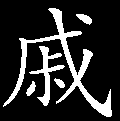
\includegraphics[width=3mm]{../Images/00005}\kaishu 总评:人谓``闹宁国府''一节极凶猛,``赚尤二姐''一节极和蔼,吾谓``闹宁国府''情有可恕,``赚尤二姐''法不容诛,``闹宁国府''声声是泪,``赚尤二姐''字字皆锋。}
